\section{Experimento 3: Red hogareña cableada}

\subsection{Descripción del contexto}

El experimento fue realizado en una red doméstica, por medio de una conexión Wi-Fi. Al momento de tomar las mediciones estaban conectados a la red varias laptops y celulares. La fecha de la captura fue Domingo 8 de Octubre de 2017.

\subsection{Descripción de la captura}

Capturamos 11000 paquetes. En la figura~\ref{protocolos4} se muestra la distribución de los protocolos en la red. Observamos que la mayoría de los paquetes son de tipo IPv4, y muchos menos son de tipo ARP y \texttt{0x86dd} (IPv6).

\begin{figure}[H]
\centering
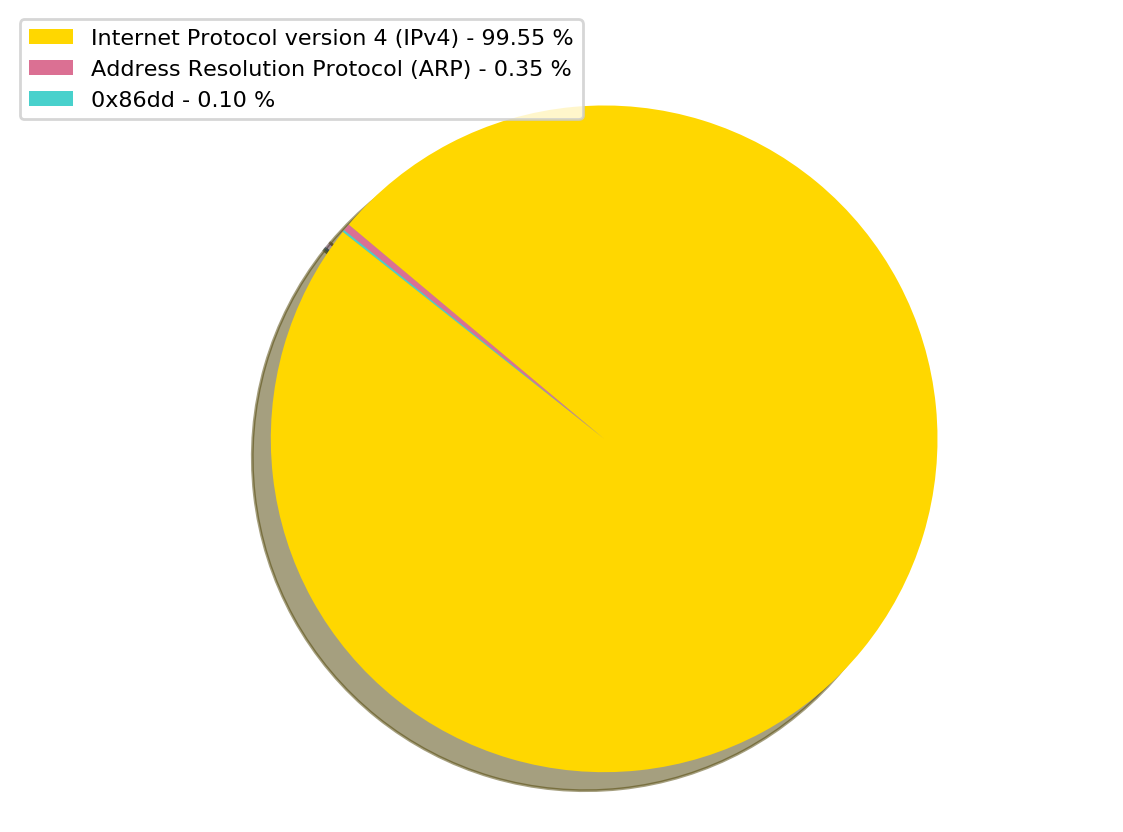
\includegraphics[width=0.7\textwidth]{protocolosRed4.png}
\caption{Gráfico que muestra la distribución de protocolos en la red.}
\label{protocolos4}
\end{figure}

En la figura~\ref{broadcast4} podemos ver el porcentaje de paquetes broadcast comparado con el total de paquetes. Vemos que esto representa un 2,2\% del total. Además, en la figura~\ref{entropias1_4} vemos que los paquetes de broadcast son de tipo IPv4 y ARP.

Este comportamiento es similar al del segundo experimento, ya que ambas son redes domésticas con pocos dispositivos conectados.

\begin{figure}[H]
\centering
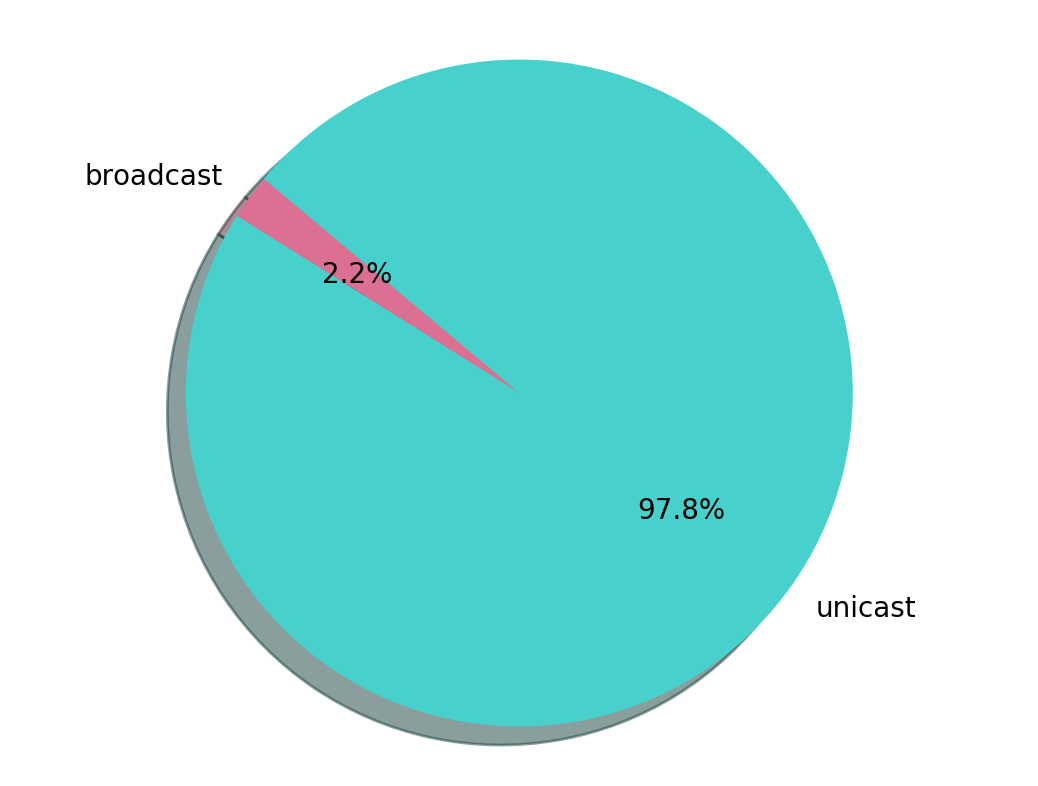
\includegraphics[width=0.7\textwidth]{broadcastRed4.png}
\caption{Gráfico que muestra los porcentajes de tráfico broadcast y unicast.}
\label{broadcast4}
\end{figure}

\subsection{Análisis de la captura}

En la figura~\ref{entropias1_4} se muestra la información de cada símbolo de la fuente S1. 
Hay un símbolo con mucha menor información que los demás (IPv4 unicast), lo cual se debe a que la mayoría de los paquetes fueron de este tipo. 
A causa de esto, la entropía de la fuente es muy baja y está muy lejos del máximo, debido a que hay grandes diferencias entre el símbolo de menor información y los demás.

\begin{figure}[H]
\centering
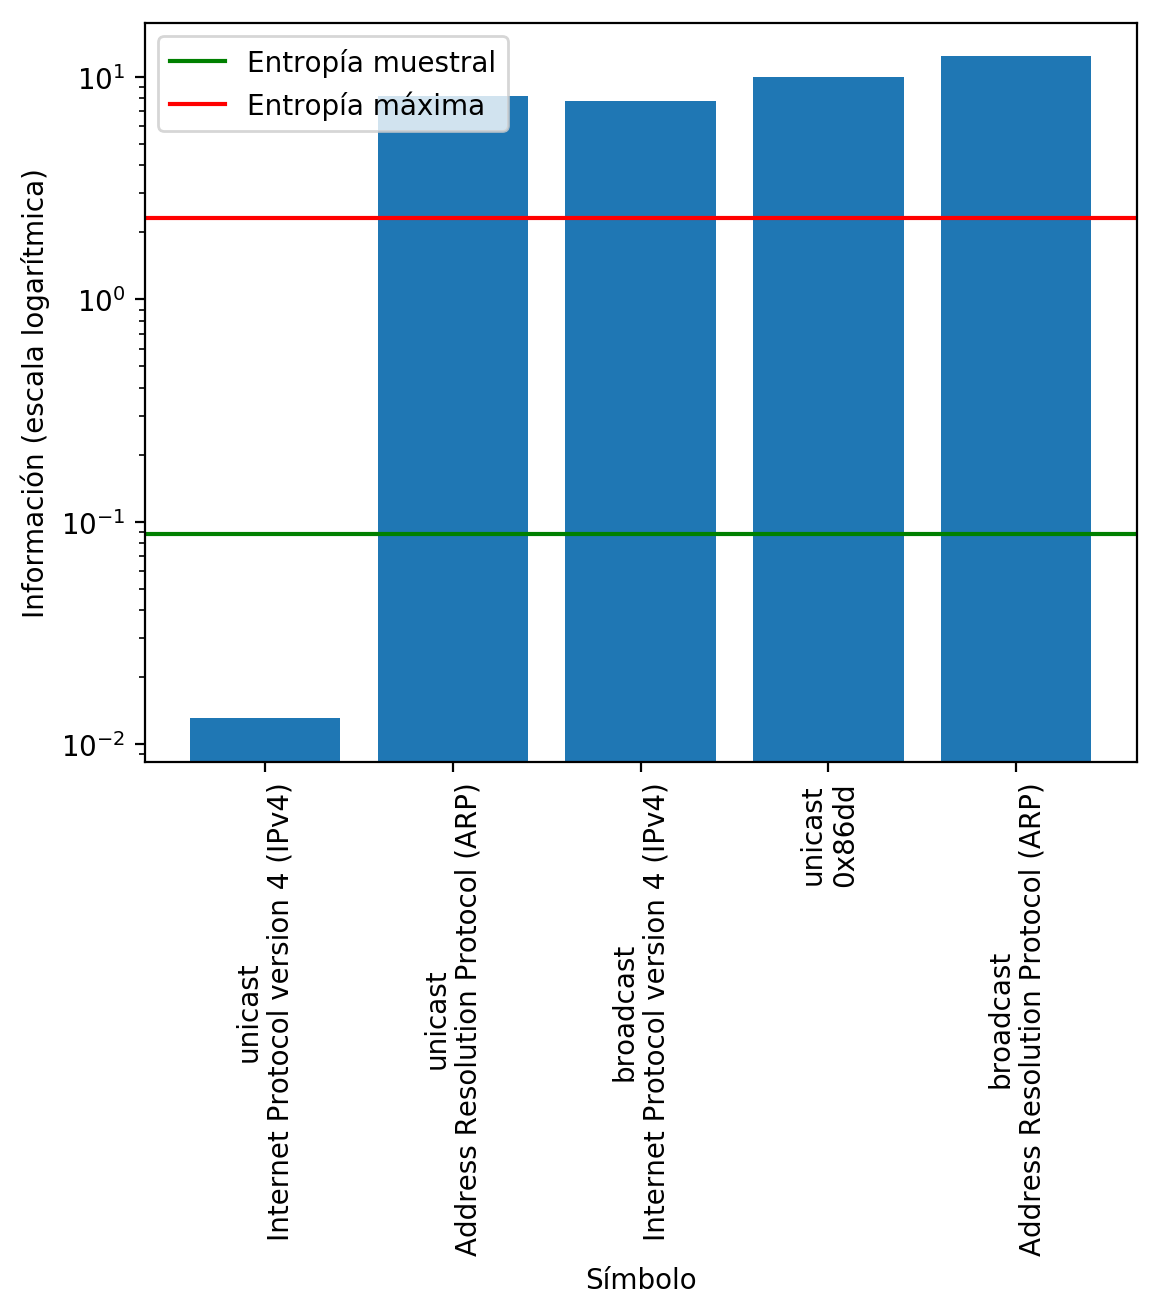
\includegraphics[width=0.7\textwidth]{entropiaS1Red4.png}
\caption{Gráfico de la información de los símbolos de la fuente $S_1$ observados en esta red. Se muestra la entropía muestral de $S_1$ y su entropía máxima.}
\label{entropias1_4}
\end{figure}

En cuanto a la fuente $S_2$, vemos en la figura 14 que sólo hay dos símbolos correspondientes a las dos direcciones IP que realizan requests ARP. Atribuimos esto a lo reducida que es la red. 
La entropía muestral está cerca de 1/2 , la mitad que la entropía máxima.

\begin{figure}[H]
\centering
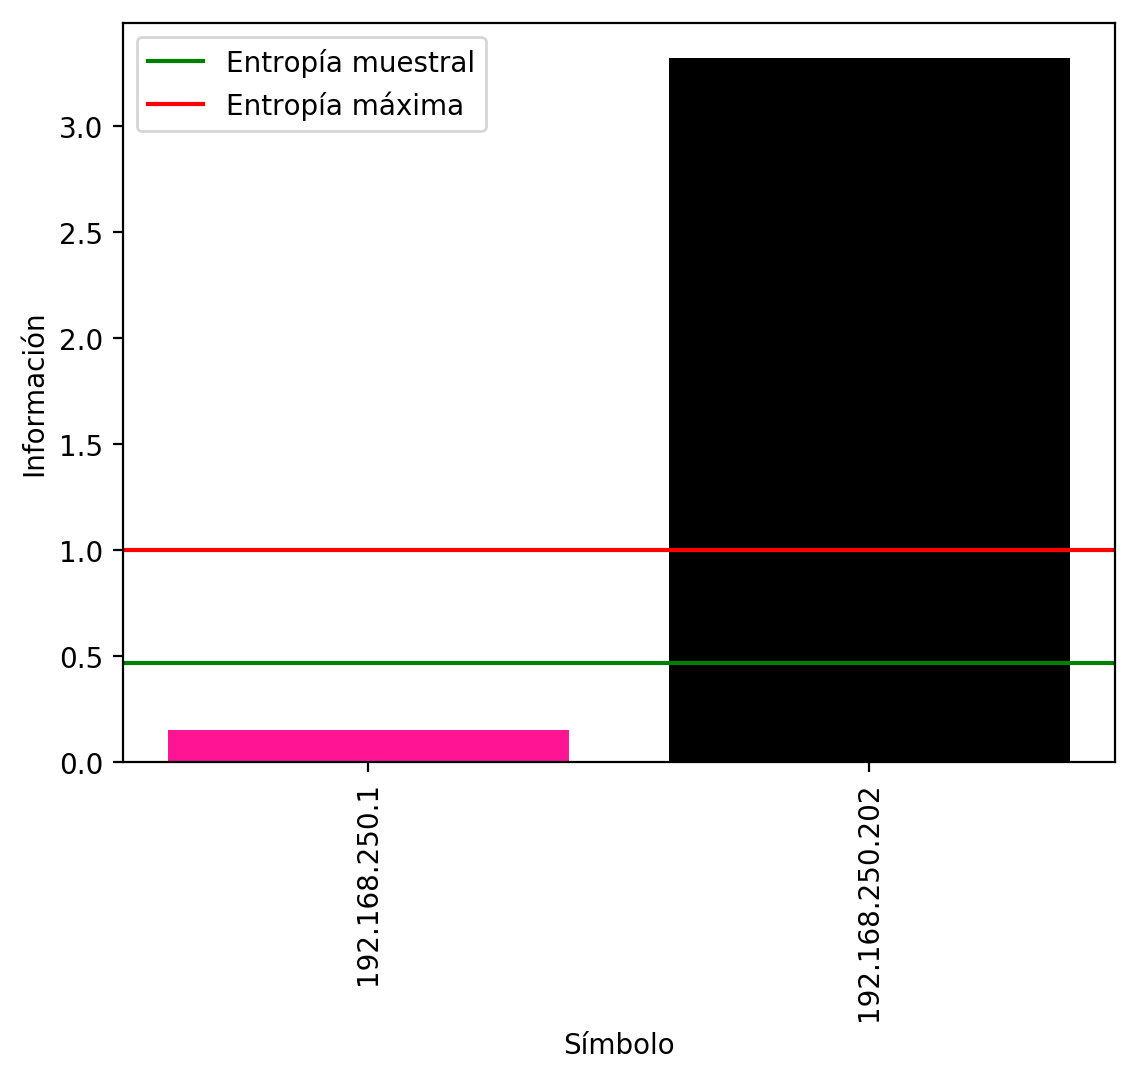
\includegraphics[width=0.7\textwidth]{entropiaS2Red4.png}
\caption{Gráfico de la información de los símbolos de la fuente $S_2$ observados en esta red. Se muestra la entropía muestral de $S_2$ y su entropía máxima.}
\label{entropias2_4}
\end{figure}

Por último representamos los envios ARP dentro de la red durante el periodo monitoreado, al igual que en los otros dos experimentos. 
Notese que aqui se representan tanto los requests ARP como sus respuestas, por lo que aparecen aqui cuatro nodos a diferencia de las dos direcciones que aparecen com simbolos de la fuente. 
Al ser una muestra sobre una red tan pequeña este grafo no muestra muchos mas aspectos relevantes para el analisis.

\begin{figure}[H]
\centering
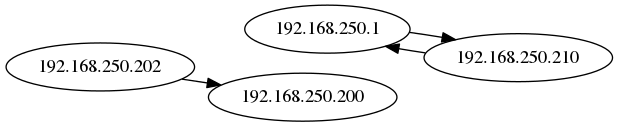
\includegraphics[width=0.6\textwidth]{grafoRed4.png}
\caption{Grafo de la red de mensajes ARP subyacente. Los nodos son las IPs observadas y los ejes son los mensajes ARP. En colores se marcan los nodos distinguidos (información por debajo de la entropía) y sus mensajes salientes. Cada arista tiene anotada la cantidad de requests/replies ARP.}
\label{grafo4}
\end{figure}